% =====================================================================================
% WHITE PAPER results (user 2026-11-12): tilts vs experiment, why MA and FA tilt oppositely, idealised processing model,
% band gap of the processed film, residual strain and thermal degradation, insights. Condensed from the full paper
% (PaperRuns/overleaf results.tex); numbers from there, energies converted to meV (1 mHa = 27.2 meV). No functional, DFT
% or force-field-training details. Figures: PaperData/paper_figs/wp_figures.py.
% CsSnI3 band gaps: preliminary (earlier calculation set) until the final CsSnI3 gaps return.
% =====================================================================================

\subsection{Do the simulations reproduce the measured structures?}
\label{sec:wp-tilts}
A process prediction is only as good as its description of the crystal, so we first test the simulations against
the measured tilts. Each compound was cooled from its cubic phase at \SI{0.25}{K/ps} and heated back at the same rate, three times, in
cells of about 2000 atoms (\SI{4.5}{nm} across); cells of \num{20000} atoms give the same results within \SI{15}{K}.
Figure~\ref{fig:wp-tilts} follows the tilt along the ramps, and Table~\ref{tab:wp-tilts} compares tilt systems, tilt
angles and transition temperatures with the measured structures.

\begin{figure}[t]
  \centering
  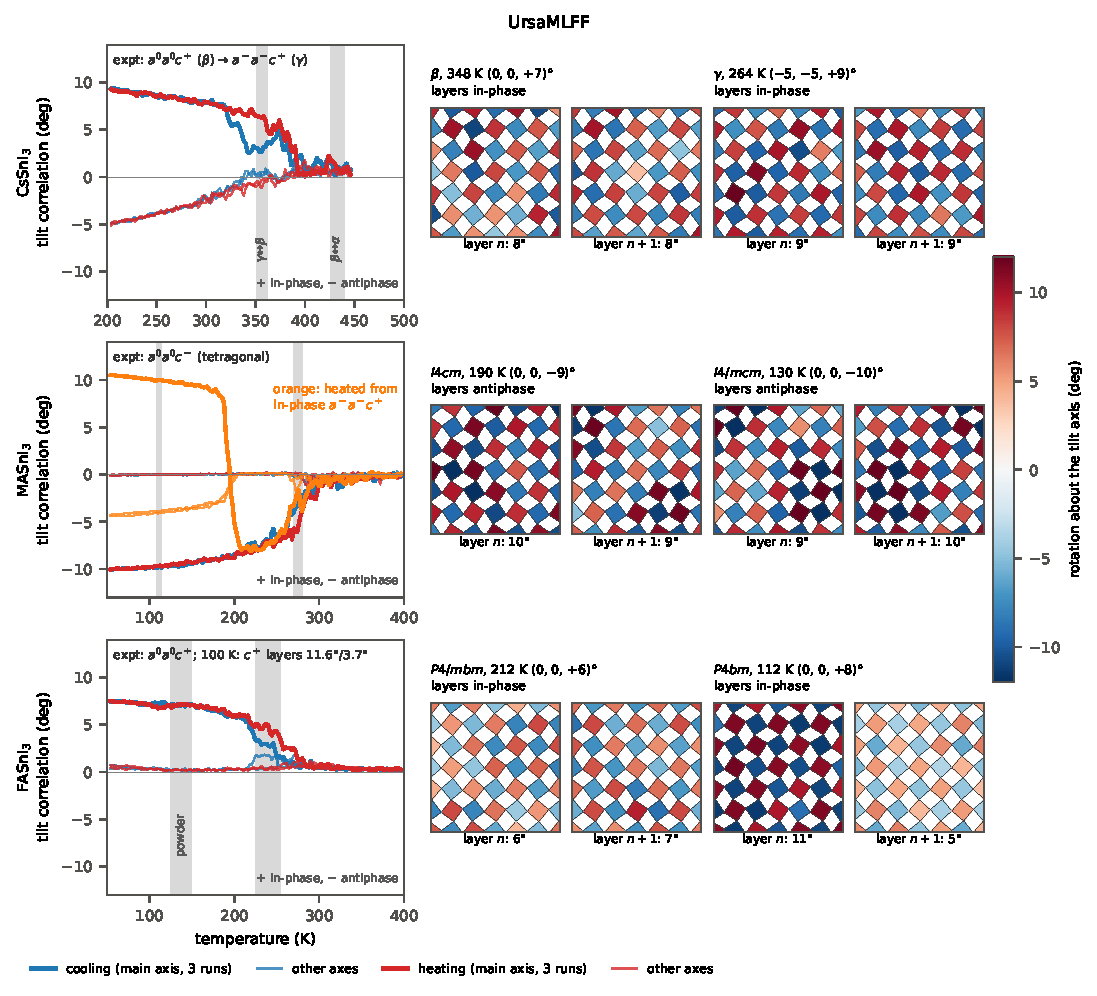
\includegraphics[width=0.74\linewidth]{wp_tiltpatterns.pdf}
  \caption{Octahedral tilts on cooling (blue) and heating (red) at \SI{0.25}{K/ps}. Left: tilt correlation of
    neighbouring octahedra about the main tilt axis (thick) and the other two axes (thin), mean of three runs; $+$
    in-phase, $-$ antiphase; grey bands: measured transitions; orange: \MASnI{} heated from an in-phase crystal. Right:
    two successive layers of octahedra in the ordered phases, each square coloured by its rotation about the tilt axis;
    in-phase stacking repeats the pattern, antiphase stacking inverts it.}
  \label{fig:wp-tilts}
\end{figure}

The simulations form the experimental tilt systems. \CsSnI{} tilts in-phase about one axis ($a^0a^0c^+$, $\beta$)
and then adds antiphase tilts about the other two ($a^-a^-c^+$, $\gamma$); \FASnI{} tilts in-phase and \MASnI{}
antiphase ($a^0a^0c^-$) in every run. The single-tilt angles agree with the measured ones to within \ang{0.3}. Below
about \SI{130}{K} \FASnI{} develops the layered tilt of its low-temperature structure, with successive layers tilted by
\ang{10.9} and \ang{4.9} at \SI{110}{K} against \ang{11.6} and \ang{3.7} measured at \SI{100}{K}. The tilt ordering of
the hybrids falls within the measured ranges, while both transitions of \CsSnI{} lie 40 to \SI{55}{K} below the
measured ones; the processing simulations below therefore place every temperature relative to the compound's own
transition.

\begin{table}[t]
  \centering\small
  \caption{Simulated (sim.) against measured (exp.) tilt systems, tilt angles and transition temperatures (heating /
    cooling). Angles: amplitude of the single tilt ($+$ in-phase, $-$ antiphase); $\gamma$-\CsSnI{}: equatorial / apical
    Sn--I--Sn bending; each compared at the same distance below its transition.\cite{Chung2012JACS,
    stoumpos2013semiconducting, Takahashi2011Dalton, Kahmann2020ACSEL, schueller2018crystal}}
  \label{tab:wp-tilts}
  \begin{tabular}{llcccc}
    \toprule
    compound & phase & tilt system & angle (deg), exp. / sim. & transition & $T$ (K), exp. / sim. \\
    \midrule
    \CsSnI{} & $\beta$ & $a^0a^0c^+$ & $+$6.0 / $+$6.2 & $\alpha\leftrightarrow\beta$ & 440, 426 / 385, 370 \\
     & $\gamma$ & $a^-a^-c^+$ & 11.3, 6.8 / 9.9, 6.7 & $\beta\leftrightarrow\gamma$ & 362, 351 / 323, 317 \\
    \MASnI{} & tetragonal & $a^0a^0c^-$ & $-$8.6 / $-$8.5 & tilt order & ${\sim}275$ / 290, 260 \\
    \FASnI{} & tetragonal & $a^0a^0c^+$ & $+$6.3 / $+$6.4 & tilt order & 225--255 / 255, 247 \\
     & low $T$ & layered $c^+$ & 11.6, 3.7 / 10.9, 4.9 & layering & 125--155 / 133, 127 \\
    \bottomrule
  \end{tabular}
\end{table}

\subsection{What sets the tilt pattern?}
\label{sec:wp-sense}
The stacking of the tilts is fixed at the first ordering transition and is inherited by the film on cooling. The
inorganic framework hardly distinguishes the two stackings, whose energies differ by about \SI{1}{meV} per formula
unit,\cite{Klarbring2019PRB} so the A-site cation must choose. We computed the free-energy difference between the
two stackings in frameworks held at the measured tilts, with only the cations moving (Figure~\ref{fig:wp-sense}b).
\FASnI{} is lower in-phase by \SI{31}{meV} per formula unit at \SI{200}{K} and by 31 to \SI{36}{meV} up to
\SI{300}{K}; \MASnI{} is lower antiphase by 15 to \SI{17}{meV}.

The cause is the shape of the cage (Figure~\ref{fig:wp-sense}a). A tilt turns each face of the cage around the
cation into a rectangle with a long axis $L$. In-phase stacking gives the lower and upper faces the same long axis;
antiphase stacking crosses them. In the in-phase cage both cations lie along the common long axis. In the crossed cage
FA, which carries an NH$_2$ group at each end and spans the cage, can follow only one face: it aligns with the far face
and lies across the near one, so one end is always squeezed (Figure~\ref{fig:wp-sense}c). MA, with a single NH$_3$
group, sits against one face and aligns with it, an arrangement that is lower in energy than in the in-phase cage.

\begin{figure}[t]
  \centering
  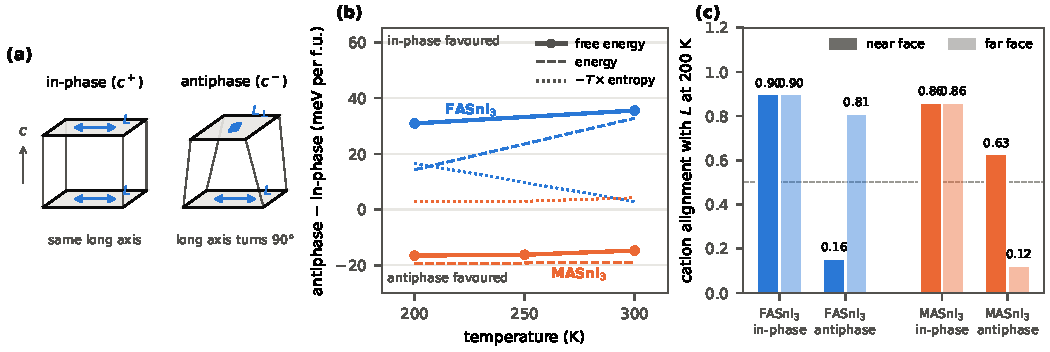
\includegraphics[width=0.9\linewidth]{wp_tilt_sense.pdf}
  \caption{Origin of the tilt stacking. (a) A tilt about $c$ makes each face of the cation cage a rectangle with long
    axis $L$; in-phase stacking keeps $L$ at the lower and upper faces, antiphase stacking turns it by \ang{90}. (b)
    Free energy of antiphase relative to in-phase stacking per formula unit, with its energy and entropy parts, in
    frameworks held at the measured tilts. (c) Alignment of the cation axis (FA N--N, MA C--N) with the long axis of the
    near and far face of its cage at \SI{200}{K}; 0.5: no preference.}
  \label{fig:wp-sense}
\end{figure}

\subsection{In which state does processing leave the film?}
\label{sec:wp-process}
With the free crystal reproduced, we add the substrate. We follow each compound through the process history of a device film: an anneal at \SI{373}{K}, cooling at
\SI{0.25}{K/ps} through the \SI{358}{K} of damp-heat testing to the operating temperature of \SI{300}{K}, and a hold
there. Each temperature is shifted by the difference between the simulated and the measured transition, so that the
film anneals and operates at the same distance from its transition as in a device. \CsSnI{} then anneals in its
$\beta$ phase and crosses into $\gamma$ during cooling, while \MASnI{} and \FASnI{} stay untilted throughout. The
substrate is described in two ways and compared with a free-standing crystal of the same history: an in-plane tension
of \SI{50}{MPa}, the measured residual stress, and an in-plane cell fixed at the end of the anneal, as for a film
bonded to a rigid substrate.

Both descriptions leave the films stretched in the plane by 0.2 to \SI{0.4}{\percent} (Table~\ref{tab:wp-film}). The
rigid substrate builds up 63 to \SI{77}{MPa}, close to the imposed \SI{50}{MPa} and to the stresses measured in
films.\cite{Rolston2018AEM, Zhao2017SciAdv, ref_processing_temp} No compound changes its tilt pattern: the constraint weakens the tilt of \CsSnI{} about the film normal from
\ang{8.5} to \ang{7.8}, and the hybrids stay untilted.

\begin{table}[t]
  \centering\small
  \caption{Processed films at the operating temperature, relative to the free crystal with the same history:
    in-plane strain $\Delta\varepsilon_\parallel$, in-plane stress $\sigma_\parallel$ (tensile positive), tilt about
    the film normal (free crystal in parentheses), and band-gap change $\Delta E_\mathrm{g}$ (mean $\pm$ standard error) of the film and of its
    purely elastic part. $^a$Preliminary.}
  \label{tab:wp-film}
  \begin{tabular}{llccccc}
    \toprule
    compound & substrate & $\Delta\varepsilon_\parallel$ (\%) & $\sigma_\parallel$ (MPa) & tilt (deg) &
      $\Delta E_\mathrm{g}$ (meV) & elastic (meV) \\
    \midrule
    \CsSnI{} & \SI{50}{MPa} tension & $+$0.40 & 50 & 8.0 (8.5) & $+$20 $\pm$ 13$^a$ & $+$18 $\pm$ 6$^a$ \\
     & rigid & $+$0.29 & 63 & 7.8 & $+$6 $\pm$ 12$^a$ & $+$19 $\pm$ 7$^a$ \\
    \MASnI{} & \SI{50}{MPa} tension & $+$0.21 & 53 & $<$1 & $+$7 $\pm$ 18 & $+$8 $\pm$ 6 \\
     & rigid & $+$0.32 & 77 & $<$1 & $+$10 $\pm$ 18 & $+$12 $\pm$ 7 \\
    \FASnI{} & \SI{50}{MPa} tension & $+$0.27 & 47 & $<$1 & $+$21 $\pm$ 20 & $+$13 $\pm$ 4 \\
     & rigid & $+$0.36 & 66 & $<$1 & $0 \pm 17$ & $+$15 $\pm$ 5 \\
    \bottomrule
  \end{tabular}
\end{table}

\subsection{Does processing shift the band gap?}
\label{sec:wp-gap}
The first device property the residual strain can change is the band gap. It was computed on snapshots of each film at the operating temperature and compared with the free crystal
(Table~\ref{tab:wp-film}). Straining free snapshots to the cell of the processed film isolates the elastic part. In
the hybrids this part opens the gap by 8 to \SI{15}{meV}; it follows the volume with a deformation potential of about
\SI{3}{eV}, as expected for a valence-band maximum of antibonding Sn 5s--I 5p character.\cite{huang2013electronic} The sign
agrees with experiment: contracting untilted FA$_{1-x}$Cs$_x$SnI$_3$ lowers its gap,\cite{Prasanna2017JACS} and in lead
halide films the more tensile surface layer emits about \SI{14}{meV} higher than the film below.\cite{Zhu2019NatCommun}
The changes of the full films agree with the elastic part, so the untilted hybrids respond elastically. At the
operating temperature the gap fluctuates by 35 to \SI{67}{meV} from snapshot to snapshot, several times the shift
caused by the process. In \CsSnI{} preliminary values give an opening of about \SI{20}{meV} under tension, again close
to the elastic part.

\subsection{Does residual strain accelerate degradation?}
\label{sec:wp-hop}
The second is the lifetime of the film. Without oxygen or moisture, the intrinsic routes of degradation are iodide migration through vacancies and, in
\CsSnI{}, conversion to the yellow phase, treated in the next section. We computed the free-energy barrier of an iodide hop into a neighbouring
vacancy at the operating temperature, with the in-plane lattice strained by $-1$, 0 and $+\SI{1}{\percent}$
(Table~\ref{tab:wp-hop}). In \CsSnI{} tension lowers both barriers, by \SI{17}{meV} per percent for hops within the
film plane and \SI{35}{meV} per percent for hops out of it; at the residual strain of a clamped film,
$+\SI{0.25}{\percent}$, iodide hops become 1.2 to 1.5 times faster. Direct simulations of cells with several
vacancies confirm the trend: at \SI{475}{K} the hop rate at $+\SI{1}{\percent}$ is $2.2 \pm 0.2$ times that of the
unstrained cell, with an activation energy of about \SI{400}{meV}. The hybrids respond less: their out-of-plane
barriers fall by 28 (\MASnI{}) and \SI{6}{meV} (\FASnI{}) per percent, their in-plane barriers are lowest under
compression, and at $+\SI{0.25}{\percent}$ their hop rates change by factors of 0.95 to 1.3. The barriers lie in the
range of measured activation energies of halide migration, $370 \pm \SI{60}{meV}$ in MASnBr$_3$\cite{Kubicki2020JACS} and
600 to \SI{680}{meV} in \ce{MAPbI3} cells.\cite{Eames2015NatCommun} Measurements on lead halide films agree in sign: the
activation energy of ion conduction in \ce{MAPbI3} films falls under tension,\cite{Zhao2017SciAdv} and tensile CsPbI$_2$Br cells degrade faster at
\SI{85}{\celsius} than compressed ones.\cite{ref_processing_temp}

\begin{figure}[t]
  \centering
  \begin{minipage}[b]{0.5\linewidth}
    \centering\small
    \captionof{table}{Free-energy barrier of an iodide hop into a vacancy (meV) against in-plane strain at the
      operating temperature; uncertainty about \SI{20}{meV}. Paths as in Figure~\ref{fig:wp-hop}.}
    \label{tab:wp-hop}
    \begin{tabular}{llccc}
      \toprule
      compound & hop & $-\SI{1}{\percent}$ & 0 & $+\SI{1}{\percent}$ \\
      \midrule
      \CsSnI{} & in-plane & 497 & 469 & 452 \\
       & out-of-plane & 409 & 373 & 338 \\
      \MASnI{} & in-plane & 333 & 392 & 397 \\
       & out-of-plane & 416 & 418 & 390 \\
      \FASnI{} & in-plane & 431 & 467 & 459 \\
       & out-of-plane & 471 & 459 & 453 \\
      \bottomrule
    \end{tabular}
  \end{minipage}\hfill
  \begin{minipage}[b]{0.46\linewidth}
    \centering
    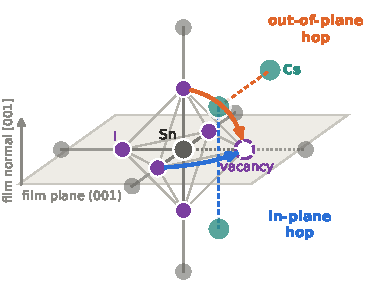
\includegraphics[width=0.78\linewidth]{wp_hop_path.pdf}
    \captionof{figure}{Iodide hop paths: from a neighbouring in-plane site or from the apical site of the same
      octahedron into an in-plane vacancy.}
    \label{fig:wp-hop}
  \end{minipage}
\end{figure}

\subsection{Can strain stabilise black \CsSnI{}?}
\label{sec:wp-yb}
Of the three compounds only \CsSnI{} has a non-perovskite competitor, a yellow phase built from chains of
edge-sharing octahedra.\cite{Chung2012JACS} Experiment fixes two points: yellow \CsSnI{} turns black only on heating,
at about \SI{425}{K}, and black films kept in air at room temperature turn yellow.\cite{Chung2012JACS,
ref_sn_instability} We computed the free energies of both phases as a function of temperature
(Figure~\ref{fig:wp-yb}). At the operating temperature the yellow phase is lower by 11 to \SI{19}{meV} per formula
unit: its lower enthalpy outweighs the larger vibrational entropy of the black phase, whose advantage grows with
temperature. The two free energies cross between 350 and \SI{385}{K}, below the \SI{425}{K} at which yellow crystals
convert on heating; the conversion rebuilds the octahedral network and sets in only above the equilibrium
temperature. The simulated yellow phase is denser by \SI{5}{\percent}, against \SI{6}{\percent} for the measured
structures,\cite{Chung2012JACS} so in-plane tension favours the black phase. The residual stress of a processed film,
50 to \SI{80}{MPa}, shifts the balance by only 2 to \SI{4}{meV} per formula unit and the crossing by 11 to
\SI{18}{K}. An in-plane strain of about \SI{1}{\percent}, the level at which substrate clamping keeps black
CsPbI$_3$ films from converting,\cite{Steele2019Science} corresponds to \SI{230}{MPa} in \CsSnI{} and moves the
crossing to 300 to \SI{335}{K}, close to the operating temperature.

\begin{figure}[t]
  \centering
  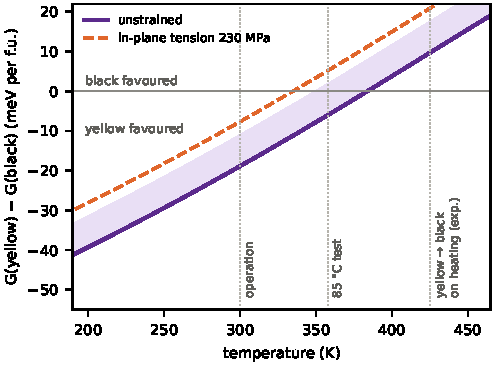
\includegraphics[width=0.48\linewidth]{wp_yb.pdf}
  \caption{Free energy of yellow relative to black \CsSnI{} per formula unit. Solid: unstrained crystal; shaded:
    uncertainty of the enthalpy difference of the two phases; dashed: in-plane tension of \SI{230}{MPa}, about
    \SI{1}{\percent} strain. Temperatures on the device scale of the processing model. Dotted: operating temperature,
    damp-heat test and the measured conversion of yellow to black on heating.\cite{Chung2012JACS}}
  \label{fig:wp-yb}
\end{figure}
